\documentclass[13pt]{extarticle}
\usepackage[utf8]{inputenc}
\usepackage{cite}

%\usepackage[margin=0.5in]{geometry}
\usepackage{textcomp}
\usepackage{longtable}
\usepackage{pgfplots}
\pgfplotsset{width=10cm,compat=1.9}
\usepackage[nottoc]{tocbibind}
\usepackage{graphicx}
\graphicspath{\images}
\usepackage{color}
\usepackage{hyperref}
\hypersetup{
    colorlinks=true,
    linkcolor=black,
    urlcolor=black,
    linktoc=all
}

\setlength{\arrayrulewidth}{.35mm}
\setlength{\tabcolsep}{18pt}
\renewcommand{\arraystretch}{1.5}
\begin{document}

%%%%%%%%%%%%%%%%%%%%%%%%%%%%%%%%%%%%%%%%%%%%%%%%%%%%%%%%%%%%%%%%%%%%%%%%%%%%%%%%%%%%%%%%%

\begin{titlepage}
	\centering
    \vspace*{0.5 cm}
    
\includegraphics[scale = 0.75]{sustlogo.png}\\[1.0 cm]	% University Logo
    \textbf{\Large Shahjalal University of Science \& Technology,Sylhet}\\[2.0 cm]	% University Name
	\textsc{\Large ProjectX Completion Report}\\[0.5 cm]				% Course Code
	\rule{\linewidth}{0.2 mm} \\[0.4 cm]
    \textsc{\Large Technical Writing}\\
	\rule{\linewidth}{0.2 mm} \\[1.5 cm]
	
	\begin{minipage}{0.5\textwidth}
		\begin{flushleft} \large
			\textbf{\textit{ Submitted To :}}\\
		     Dr. Ahsan Habib\\
		     Assistant Professor\\
            Dept. of Software Engineering(IICT),SUST\\
			\end{flushleft}
			\end{minipage}~
			\begin{minipage}{0.4\textwidth}
            
			\begin{flushright} \large
			\textbf{\textit{Submitted By :}} \\
			Mutasim Billah Toha\\
            Reg.No. : 2017831018\\
            Dept.of Software Engineering(IICT),SUST
		\end{flushright}
	\end{minipage}\\[1.3 cm]
    20 february, 2021\\
\end{titlepage}

%%%%%%%%%%%%%%%%%%%%%%%%%%%%%%%%%%%%%%%%%%%%%%%%%%%%%%%%%%%%%%%%%%%%%%%%%%%%%%%%%%%%%%%%%
\pagebreak

%%%%%%%%%%%%%%%%%%%%%%%%%%%%%%%%%%%%%%%%%%%%%%%%%%%%%%%%%%%%%%%%%%%%%%%%%%%%%%%%%%%%%%%%%
\tableofcontents

\newpage
\section{\textbf{Project Idea:} }

\quad X ( Business Holder) wants to open a new delivery service on his locality. He thinks it has great potential and is profitable. He has arranged some local drivers who will be carrying goods door to door. Now for marketing, he uses social media for publicity. His business operation is based on phones. He receives orders over the phone. Then send a photo of the order to one of his currently available drivers. The driver, later on, collects items and carries them to the customer’s home. Finally, the customer checks every item and the bill for the order and pays for the service. 

Y (Customer) thinks he can use X’s service. This service will save him time. He really does not want to visit crowded local bazar at this hot and humid weather. But he finds it difficult to connect one of the phone numbers provided by X. Y is hoping X will start taking orders from apps or sites. It would be much better for him. 

 So what we want to provide X is a web platform where his customers will place orders. If they prefer over phones then X will initiate a new order for his service, where he will place an order on behalf of his customers. This service will generate a better invoice which X will send to his employee. At the end of the day, it will be easier for X to keep track of his daily business. Moreover, this can help X’s business to grow better. And X will use this provide as pay peruse. We will be taking care of his all technical issues. 

We can provide this service to any local delivery business around the country.
\newpage
\section{\textbf{Project Summary:}}
\subsection{Project Background:}
\quad The ongoing problem for a customer and business-holders is unable to connect with one-another instantly and connecting takes too long.Besides,there is no list of orders which is done by traditional way like over phone or offline.Business holder also can not keep the track of business by the traditional way.It is also quite impossible for a business holder to extend his business area because of the distance from his shop.Customers also unable to take better services because of the distance of the shop which give better service.Both customers and business holders have to worry about the ongoing problem because of their own interest.
\subsection{Project Objectives:}
\begin{enumerate}
  \item Connecting customers and business holders instantly.
  \item Keeping history of orders for both business holder and customers.
  \item Keeping the track of delivery-man for giving wide services.
  \item Generating invoices for the customers and business holders.
  \item Getting more audience through internet so that both business holders and customers can have better service.
\end{enumerate}
\newpage

\section{\textbf{Requirements:}}
\subsection{Use Case Diagrams}
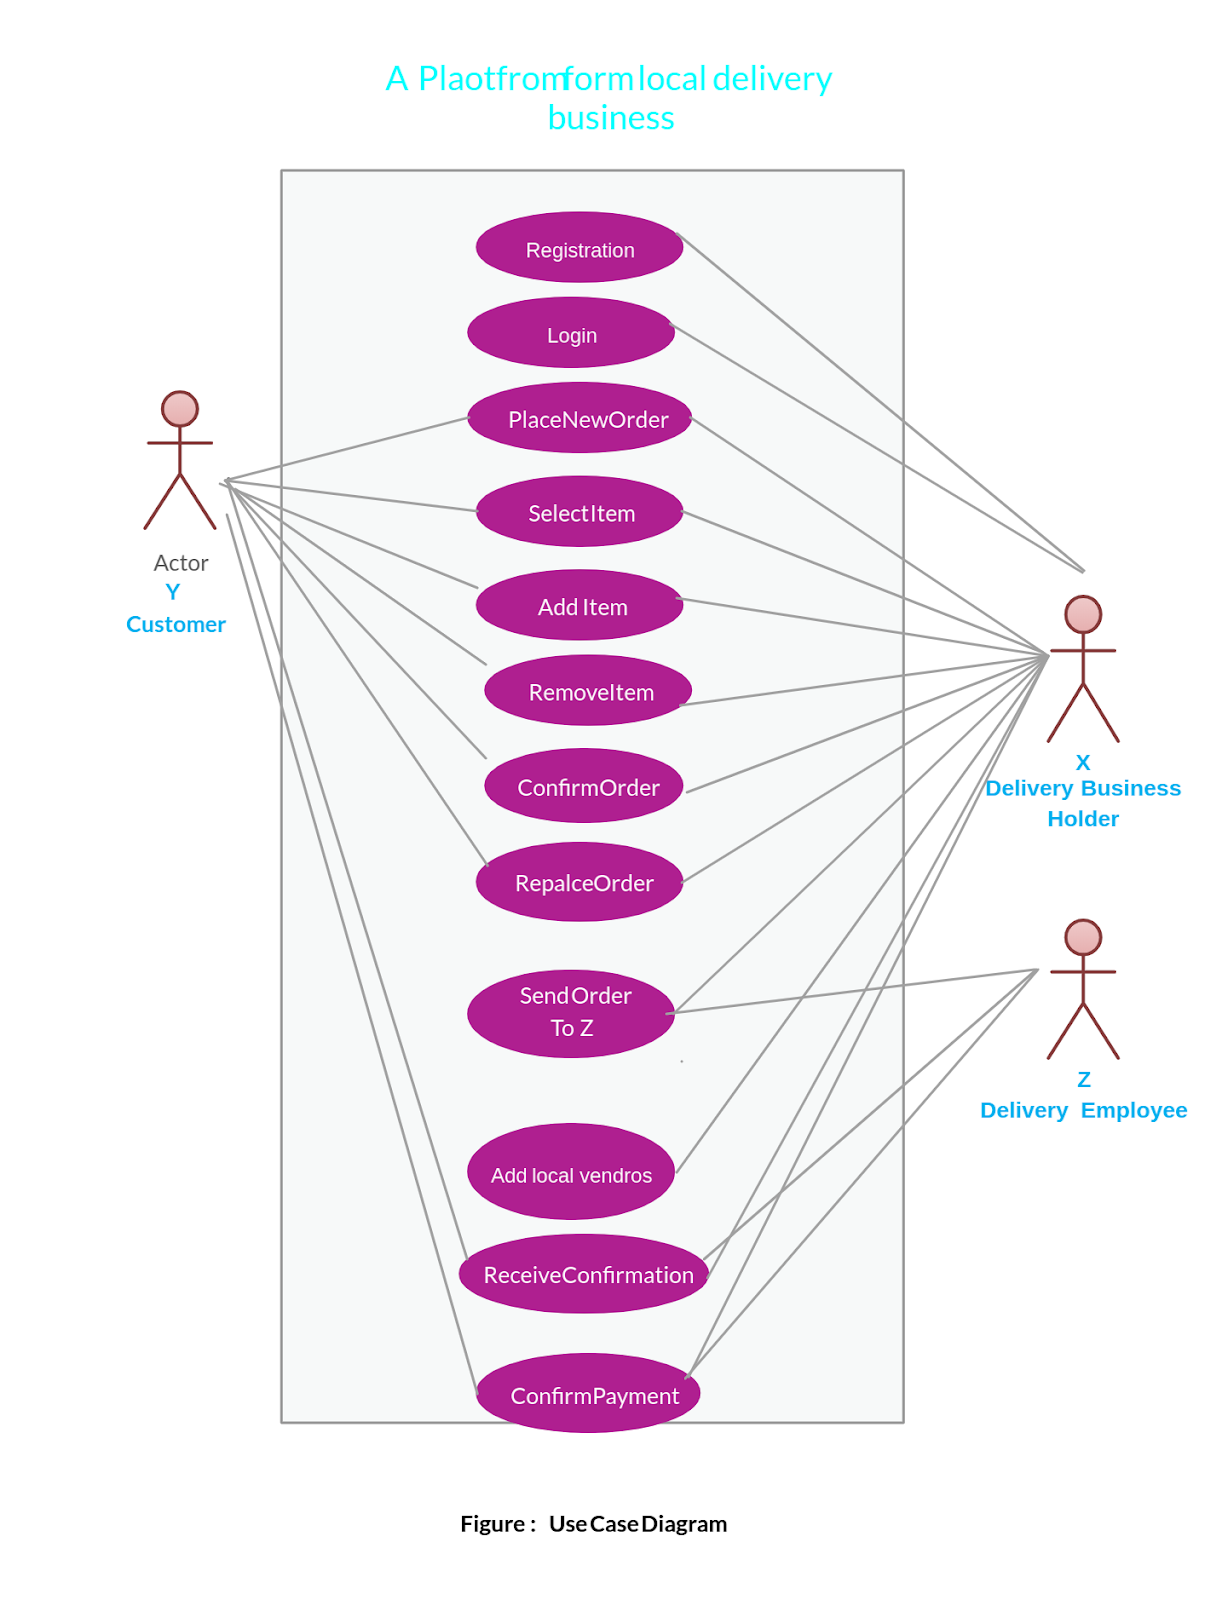
\includegraphics[scale = 0.25]{usecase.png}\\[1.0 cm]	
\newpage
\subsection{Functional Requirements}
\subsubsection{Business Holders:}
\begin{itemize}
    \item Registration/login 
    \item Update Profile
\item Receives Order from customers
\item Initiate Order for customers
\item Create Services ( Laundry, Grocery, Ticket, Medical Report)
\item Manage Business
 \item Generate invoice 
 \item Inventory
 \item History
\end{itemize}
\subsubsection{Customers:}
\begin{itemize}
    \item Registration/login 
    \item Update Profile
\item Select services ( Laundry, Grocery, Ticket, Medical Report)
\item Select preferable local vendors ( Local service providers) 
\item Place new Order
\item History of previous orders
\end{itemize}
\newpage
\subsection{Non-Functional Requirements}
\subsubsection{Usability}
Upon authentication, customer can create an order function in two-three clicks.
\subsubsection{Security}
Only a certain category of users may access data on payments and transactions.
\subsubsection{Scalability}
The website should be able to support 500 users simultaneously.
 \subsubsection{Performance}
Website page load time should not exceed 2 seconds.
 \subsubsection{Availability}
Service downtime shouldn’t exceed 20 minutes. The users should be redirected to a front website page during the downtime period. 
 \subsubsection{Portability and compatibility}
The website should work with all kind of operating systems and browsers. 
 \subsubsection{Appearance}
 The software shall comply with corporate branding standards.The product shall be attractive to a teenage audience.
 \newpage
\section{\textbf{Achievement of Project Purpose:}}
\begin{center}
Planned vs Actual Performance\\
\begin{tabular}{ |p{5cm}|p{5cm}|  }
\hline
\multicolumn{2}{|c|}{Achievement} \\
\hline
Indicator & Actual at Completion\\
\hline
faster to order for customers & Achieved.Customers can order from any service service providers less than one minute.The process of creating an order is so easy for a new customer.\\
\hline
Better and easier communication between business holders and customers & Achieved.Customer can easily contact to the service providers as he/she can see the providers' info while ordering.Service providers also can see the customer info while collecting orders.Later,they can contact each other with the info if needed.\\
\hline
Transparency in pricing & Achieved.Service providers and customers can see the pricing of the product on the website properly and there is no hidden charge for the customers.\\
\hline
Less cost in communicating and ordering & Achieved.Customers can simply create an order and can contact with the service provider if any special instruction is needed and vice versa.\\
\hline
Better system for monitoring the business for holders & Achieved.Service providers can see the statistics of their sell between dates which help them to supervise their business. \\
\hline
\end{tabular}
\end{center}
The software fulfils all the expectations according to the purpose of this software.According to the project proposal, the software should work given on the functional and non-functional requirements.And after completing the software implementation, it matches with all functional and non-functional requirements and gives the correct output.So, we can say that the software achieves all the project purposes.There are no unexpected behavior from the software.
\newpage
\section{\textbf{Project Output:}}
\begin{center}
Requirements,Expected Output and Actual Performance of the software is shown below
\begin{longtable}{ |p{2.5cm}|p{4cm}| p{4cm}| }
\hline
Requirements& Expected Performance & Actual Performance\\
\hline
\multicolumn{3}{|c|}{Customer Side} \\
\hline
Registration & Customers can register on the website giving his username and phone number & Achieved.By giving username and correct phone number customers can successfully register in the website.\\
\hline
Login & Customers can login with the phone number given on the registration process & Achieved.Customers can login with the number given in the registration process.\\
\hline
OTP & Customers should get an otp on their registered phone number & Achieved.Server sends otp to the registered number of a customer.\\
\hline
Update Profile & Customers can update his/her profile after successfully logged in & Achieved.Customers can update his username in the update profile option only when he/she is successfully logged in.\\
\hline
Selecting Local Vendors & Customers can select his local vendors by selecting his location from drop down box and can see all type of local services in his areas & Achieved.Customers can select his local address from the drop down box and can see the local vendors and can select the services given by the local vendors.\\
 \endfirsthead
\hline
Cart & Customers can see the products he/she selected from the local vendors and can checkout from the cart.He can see all the expenses and can remove the products he unintentionally selected. & Achieved.Customers can see the products in cart and can see the price of the products and their amount and can remove any product.He also can go to checkout and can do more shopping from the website if he/she intends to do so.\\
\hline
Checkout & Customers can see the products he/she selected from the local vendors and he can add address in the checkout page or can select the previous addresses he used for an order in previous.He can see all the expenses. & Achieved.Customers can see the products in checkout and can see the price of the products and their amount.He can add address or select any previous address he used.He also can add description for the delivery guy.\\
\hline
History & Customers can see all the previous orders & Achieved.Customers can see all previous orders.He can see the payment amount and can see the products' details and their amount.He can also see the used address for his orders.\\
\hline
Theme & Customer can change his theme between light or dark & Achieved.There are two theme in the website which are dark and light.\\
\hline
\multicolumn{3}{|c|}{Service Provider Side} \\
\hline
Registration & Service providers can register on the website giving his username,phone number,NID number,Trade License Number,Service Type,Delivery Charge,Descriptions & Achieved.By giving the required info service providers can successfully register in the website.\\
\hline
Login & Service providers can login with the phone number given on the registration process & Achieved.Service providers can login with the number given in the registration process.\\
\hline
OTP & Service providers should get an otp on their registered phone number & Achieved.Server sends otp to the registered number of a service provider.\\
\hline
Update Profile & Service provider can update his/her profile after successfully logged in & Achieved.service providers can update his info in the update profile option only when he/she is successfully logged in.\\
\hline
Orders & Service Provider can see all the orders he got and can complete his order by actions & Achieved.Service provider can see all the orders and necessary details for the orders like customer address,phone,ordered time.He/She also can see the product details in the order list. 
\hline
History & Service providers can see all the previous orders he/she delivered & Achieved.Service providers can see all previous orders.He can see the payment amount and can see the products' details and their amount.He can also see the customers' address for the orders.\\
\hline
Statistics & Service provider can see the number of orders he got between two dates,he/she can see the number of delivered orders and can see the total income & Achieved.Service provider can see the number of orders he got between dates,can see the number of delivered orders and can see the total income.\\
\hline
Add Product & Service providers can add product in his inventory & Achieved.Service providers can add product with product name and its price.\\
\hline
Inventory & Service provider can see his/her inventory and can update any product details or can remove any product from his/her inventory & Achieved.Service provider can see the inventory and can update or remove any item from the inventory/\\
\hline
Service Area & Service providers can extend the area of his delivery or can shorten the area he/she wants to deliver & Achieved.Service provider can add more area or remove from his delivered area. \\
\hline
Employee & Service provider can add or remove or update his own employee & Achieved.Service provider can add/remove/update his employee list.\\
\hline
Theme & Service provider can change his theme between light or dark & Achieved.There are two theme in the website which are dark and light.\\
\hline
\end{longtable}
\end{center}
\section{\textbf{Lessons learned from the project:}}
\begin{itemize}

\item Development resources, used throughout the project, were rather inadequate.
\item Overall project goals and requirements could not be frozen early enough.
\item  Start small, then extend.
\item Add logging and error handling early.
\item Test the parts before the whole.
\item  Everything takes longer than one think.
\item First understand the existing code.
\item  Fix the known errors, then see what’s left.
\item Finally, Keep learning.
\end{itemize}
The result — as the software itself goes — turned out to be according to the goals and expectations. The experience gained in the area of project management is still being distilled.
\newpage
\section{\textbf{Success of the project:}}
As there were clear objectives and requirements for the website,it was easier to get the output as intended.More documentation can increase any software's or project's success rate.To start a project, there must be a plan before executing the project.There could be change in the middle of project but there should always be a plan.To avoid any unwanted output,one should follow the best practices.As the website was built while keeping this details in the head,it can be said that the project was successful.It matches all the expectations from the requirement and performs accordingly as intended.We rate it overall as an outstanding success.
\section{\textbf{Next Steps:}}
Some features can be added in the next development phase.\\
\subsection{Customer Side:}
\begin{itemize}
    \item GPS order tracking:The ability to track the current location of package and the time of arrival using location services could be added.
    \item In-app messaging : integration with phone calls is needed to re-schedule the delivery or contact the driver after the order has been accepted.
    \item Rating system: The ability to rate the courier and leave feedback.
    \item Push notifications for cases when the order is on the way or has arrived
\end{itemize}
\subsection{Service Provider Side:}
\begin{itemize}
    \item In-app messaging: for communication with the customers.
    \item Delivery status: A delivery man can update the customer when he has accepted/rejected the order, picked it up and delivered.
    \item Ratings and feedback: For complete transparency, not only the customers, but the service providers should also be able to rate their customers and leave feedback about the order.
\end{itemize}
\newpage
\begin{thebibliography}{9}
\bibitem{}
 \href{https://nodejs.org/en/docs/}{https://nodejs.org/en/docs/}
\bibitem{}
\href{https://dev.mysql.com/doc/}{https://dev.mysql.com/doc/}
\bibitem{}
\href{https://cloud.google.com/docs}{https://cloud.google.com/docs}
\bibitem{}
\href{https://reactjs.org/docs/getting-started.html}{https://reactjs.org/docs/getting-started.html}
\bibitem{}
\href{https://docs.github.com/en}{https://docs.github.com/en}
\bibitem{}
\href{https://expressjs.com/en/resources/glossary.html}{https://expressjs.com/en/resources/glossary.html}
\bibitem{}
\href{https://www.twilio.com/docs}{https://www.twilio.com/docs}
\end{thebibliography}
\end{document}


\hspace{1 cm}
\begin{center}
\textbf{The End}
\end{center}
\newpage
\end{document}